% Artyom Voronin
%           _                     
% _ __ ___ | |__  _ __  _ __ ___  
%| '_ ` _ \| '_ \| '_ \| '_ ` _ \ 
%| | | | | | |_) | |_) | | | | | |
%|_| |_| |_|_.__/| .__/|_| |_| |_|
%                |_|              
%
% Brno, 2021


\chapter{PdM using a Simulation Model}\label{ch:mb}
This chapter deals with model-based methods and the possibilities of using
a simulation model to design and develop a PdM algorithm.  Section
\ref{sec:diffs_mb_dt} presents the difference between model-based PdM and
PdM using the simulation model as a digital twin.  A demonstration of the
possibility of generating sensor fault conditions is demonstrated in
section \ref{sec:sensor_fault_generation}.  Using identified
Hammerstein-Weiner model to extract condition indicators in the form of a
dynamic system parameter shown in section \ref{sec:mb_hw_demo}.  In section
\ref{sec:residuals}, the simulation model is used as a nominal, and
residual estimation is performed with the following training of the
classification model.  The left sections \ref{sec:mb_rul} deal with the use
of a simulation model to generate degradation data. And the use of a newly
generated dataset to estimate the remaining useful life.


\section{Differences between Model-Based PdM and PdM using Digital Twin}\label{sec:diffs_mb_dt}
There is a difference between using Model-Based PdM and using Simulation
Model as a Digital Twin.

\section{Using Simulation Model to Generate Fault Data}\label{sec:sensor_fault_generation}
In this section, the simulation model will play the role of a digital twin
for experimenting.  Digital Twin can be used to model situations that did
not capture in the original dataset or if it is hard to model some cases
with real-world hardware.

As an example, we can model sensors fault such as
sensor drift or complete signal loss. Suppose the simulation model signal
is in good agreement with the real-world system. In that case, the
generated data can complement the primary dataset, introducing a more
significant number of observed fault situations.



\subsection{Sensor Fault Modeling}

Three basic situations measuring the nominal behavior of the system were
simulated. By adding measurement noise to the system, a "noise" fault
situation was created. Another modeled case was made using the offset.  In
Figure \ref{fig:mb_sensor_faults_signal}, flow sensor fault condition
signals are generated. This straightforward situation illustrates the
possibility and simplicity of performing experiments with a simulation
model to develop robust PdM algorithms.

\begin{figure}[h!]
    \centering
    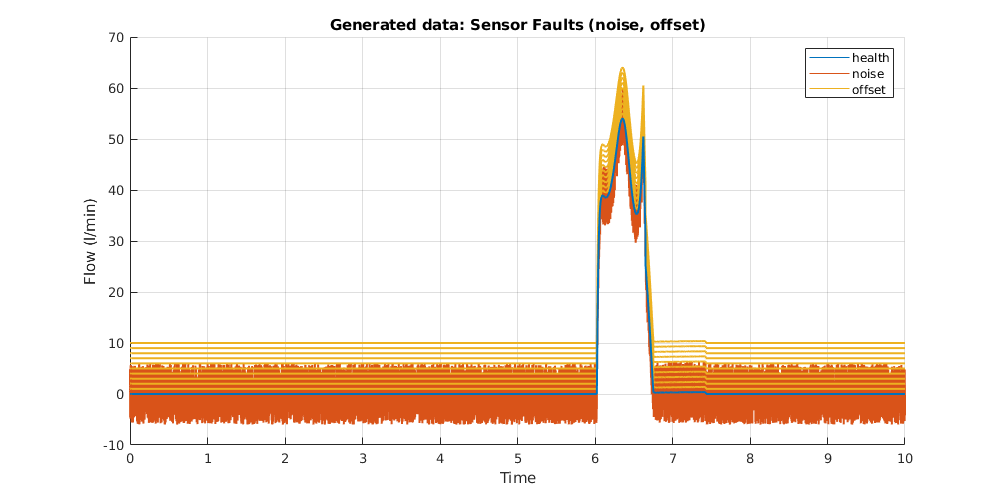
\includegraphics[width=1\textwidth]{mb_sensor_signal.png}
    \caption{Sensor response in different fault conditions}
    \label{fig:mb_sensor_faults_signal}
\end{figure}


The matrix of Scatter plots grouping by faults \ref{fig:mb_sensor_matrix} shows how condition
indicators are distributed. The data are well separable, which means that
these condition indicators are suitable for use in classification. The
confusion matrix \ref{fig:mb_sensor_conf} provides 100 \% accuracy on test data. Which in this
simplified situation is possible. In more complex cases, achieving 100 \% is
practically impossible, but it is possible to get close.

\begin{figure}
    \centering
    \begin{subfigure}[b]{0.45\textwidth}
        \centering
        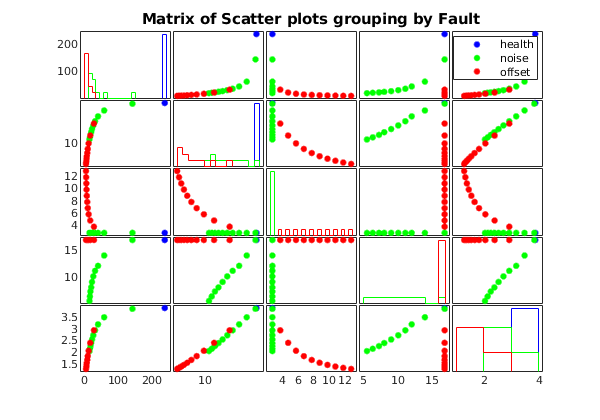
\includegraphics[width=1.2\textwidth]{mb_sensor_matrix.png}
        \caption{Sensor fault condition indicators distribution}
        \label{fig:mb_sensor_matrix}
    \end{subfigure}
    \hfill
    \begin{subfigure}[b]{0.45\textwidth}
        \centering
        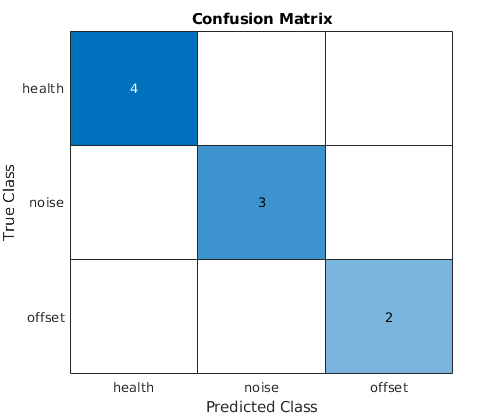
\includegraphics[width=1\textwidth]{mb_sensor_conf.png}
        \caption{Confusion matrix test dataset}
        \label{fig:mb_sensor_conf}
    \end{subfigure}
    \caption{Classification performance}
    \label{fig:sensor_fault_final}
\end{figure}



\section{Model-Based Condition Indicators}
The model-Based approach is suitable when it's challenging to identify
condition indicators using only signals. In some cases, it's useful to fit
some models from data and extract condition indicators as some system
parameter.

\paragraph{Static models}
If the system behavior can be identified from the data as a static model,
we can extract condition variables from this model as model parameters. For
example, if the model is fitted to a polynomial model, polynomial
coefficients can be used as condition indicators.

\paragraph{Dynamic models}
Signals showing dynamic behavior can be identified as dynamic models such
as State-Space or AR, ARX, NLARX (Nonlinear auto recursive model), and so
on.  Then condition indicators can be extracted as poles, zeros damping
coefficients from the identified model.

\paragraph{State obesrvers}
Another possibility is to use the Kalman filter and other state observers
to estimate all state variables from the measured signal. It is suitable if
the system's condition is directly dependent on some state variable that is
difficult to measure directly.

\subsection{Using Hammerstein-Wiener Model}\label{sec:mb_hw_demo}
In this demonstration, the Hammerstein-Wiener Model was used to identify
the system using position measurement \ref{fig:mb_hw_workflow}. A smaller
data set was used for the experiment, which contains 660 measurements, six
primary fault states. An HW model was identified for each signal position.
Condition indicators were extracted in the form of a system coefficient,
both a linear block and an input/output layer.

The training of the classification model was unsuccessful, and the
resulting accuracy did not exceed 40 \%. Therefore, I consider this
approach inappropriate in this particular case.

\begin{figure}[h!]
    \centering
    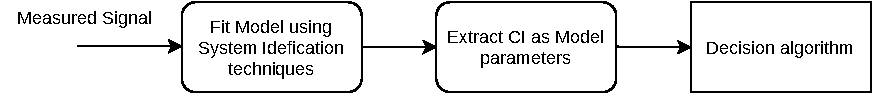
\includegraphics[width=0.8\textwidth]{mb_hw.pdf}
    \caption{Using identification model for PdM workflow}
    \label{fig:mb_hw_workflow}
\end{figure}


\section{Using Simulation Model for Residuals Estimation}\label{sec:residuals}
The residual Estimation approach is another option to use a simulation
model to achieve fault detection.  The residual is a subtraction of two
signals in the form $e(t) = y(t) - \hat{y}(t)$ as shown in
\ref{fig:mb_resid_workflow}.

\begin{figure}[h!]
    \centering
    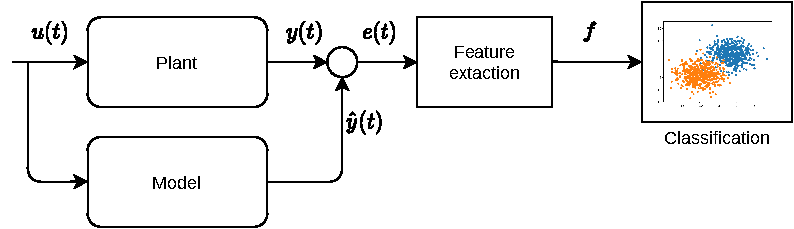
\includegraphics[width=0.7\textwidth]{mb_resid.pdf}
    \caption{Residual estimation diagram}
    \label{fig:mb_resid_workflow}
\end{figure}

Residual estimation can be helpful when the system response is highly
dependent on the input signal, and the measured dataset does not observe
all possible faults. Residuals are very sensitive detectors of problems. In
some cases where the system changes operation conditions but still operates
in a healthy state and this change does not reflect the nominal simulation
model, the decision algorithm may signalize a fault. This type of fault,
also known as false positive, indicates problems that do not exist \cite{}.
Generally, this approach requires a smaller amount of data for training the
classification model. It is very suitable for system monitoring, where if
the residual of two signals outreaches any given threshold, a fault state
has occurred. 



To demonstrate residual estimation and save calculation time, a smaller
dataset was used. Since the signals represent the same 10-second intervals,
the simulation was performed only once and then used as the nominal
reference behavior for all calculations of all residuals. However, for
deploying this algorithm, the simulation model runs in real-time and
continuously generates residuals.

\begin{figure}[h!]
    \centering
    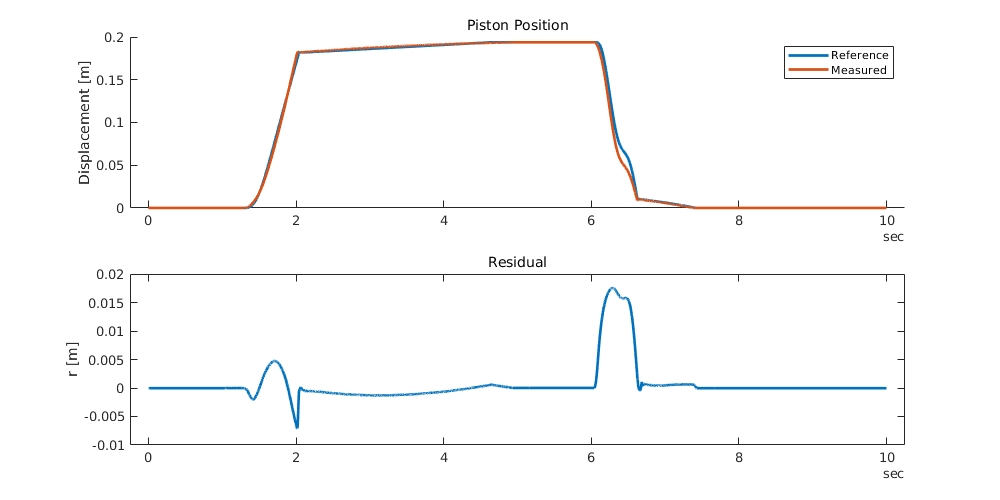
\includegraphics[width=1\textwidth]{mb_resid_signal.png}
    \caption{Residual signal of measured and simulated position}
    \label{fig:mb_resid_signal}
\end{figure}

A linear encoder was used as an example. Figure \ref{fig:mb_resid_signal} shows the residual
for the measured and reference signal. These residual signals were then
combined to the dataset from which condition indicators were extracted as
statistical parameters.  Using the same steps described in the signal-based
example \ref{sec:flow_example}, condition indicators were ranked
\ref{tab:resid_sorted_ci}, and the
classification model was trained. The trained classification model shows
excellent accuracy of 99.49 \%. Predictions are shown in confusion matrix
\ref{fig:mb_resid_conf}.

\begin{table}[h!]
    \centering
    \begin{tabular}{|c|c|c|}
        \hline
          &        Features               & Kruskal-Wallis \\ \hline
        1 &   LeverPosition\_res\_stats/RMS	    & 543.82 \\ \hline  
        2 &   LeverPosition\_res\_stats/PeakValue	& 271.94 \\ \hline  
        3 &   LeverPosition\_res\_stats/Std	    & 222.89 \\ \hline  
        4 &   LeverPosition\_res\_stats/THD	    & 215.34 \\ \hline  
        5 &   LeverPosition\_res\_stats/Kurtosis	& 129.66 \\ \hline  
    \end{tabular}
    \caption{First Five Ranked Condition Indicators using ANOVA}
    \label{tab:resid_sorted_ci}
\end{table}

\begin{figure}[h!]
    \centering
    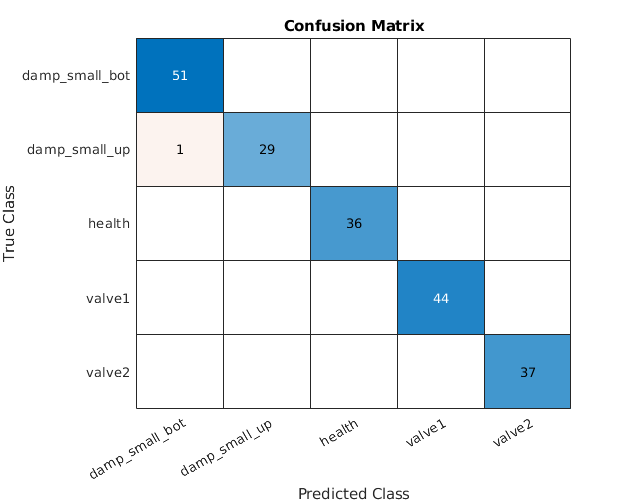
\includegraphics[width=0.7\textwidth]{mb_resid_conf.png}
    \caption{Classification model perfomance}
    \label{fig:mb_resid_conf}
\end{figure}

For comparison using the signal-based method applying to the same dataset,
classification results are similar 99.49 \%.
By given the results, the residual estimation method may seem unnecessary.
In this particular case, from a practical point of view, there is no
improvement of the result, but the calculation time increases
significantly. 


\section{Using Simulation Model to Generate Prognostic Data}\label{sec:mb_rul}
Another option is to use a simulation model to simulate a system degradation
process. We can evaluate CI from sensor signal by changing a system's
mechanical properties as friction or mass flow leakage.  Another advantage
is that we can design experiments on the model to evaluate what type of
data we require from a real-world system to develop a robust algorithm.

\subsection{Air Leak Modeling}
\begin{figure}[h!]
    \centering
    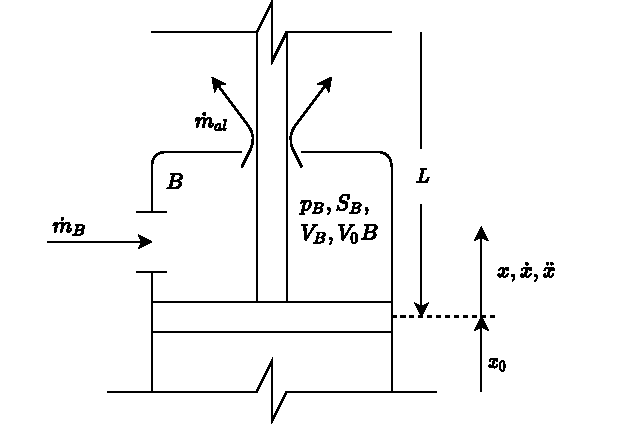
\includegraphics[width=0.4\textwidth]{air_leak.pdf}
    \caption{Schematic representation of the air leak process}
    \label{fig:air_leak_scheme}
\end{figure}

One of the common failures in pneumatic actuators operation is air leakage
from the chamber where the piston is located. Dust and other contaminants
can damage the connection between the cylinder and the piston, causing air
leakage. This problem is schematically illustrated in Figure
\ref{fig:air_leak_scheme}.


In this example, air leakage from the chamber was modeled the same as air
expansion from the reservoir, described in section \ref{sec:}.  Due to the
notation in Figure \ref{fig:air_leak_scheme}, the air leakage process
describes equation \ref{eq:air_leak_flow}.

\begin{equation}
    \dot{m}_{al} = C_{al} p_B \sqrt{\frac{2}{R T_B}} \cdot
    \psi\left( \frac{P_0}{P_B} \right)
    \label{eq:air_leak_flow}
\end{equation}

Air leakage is reflected in the pressure in chamber B according to the
equation \ref{eq:p_B_rul}.
\begin{align}
    \dot{p_B} = \frac{\kappa}{S_B (L-x) + V_{0B}} \left(p_B S_B\dot{x} +
    RT_B[\dot{m_B}-\dot{m}_{al}] \right)
    \label{eq:p_B_rul}
\end{align}

Figure \ref{fig:pressure_air_leak} shows the development of pressure in the
chamber without air leakage and with a very significant leakage value.

\begin{figure}[h!]
    \centering
    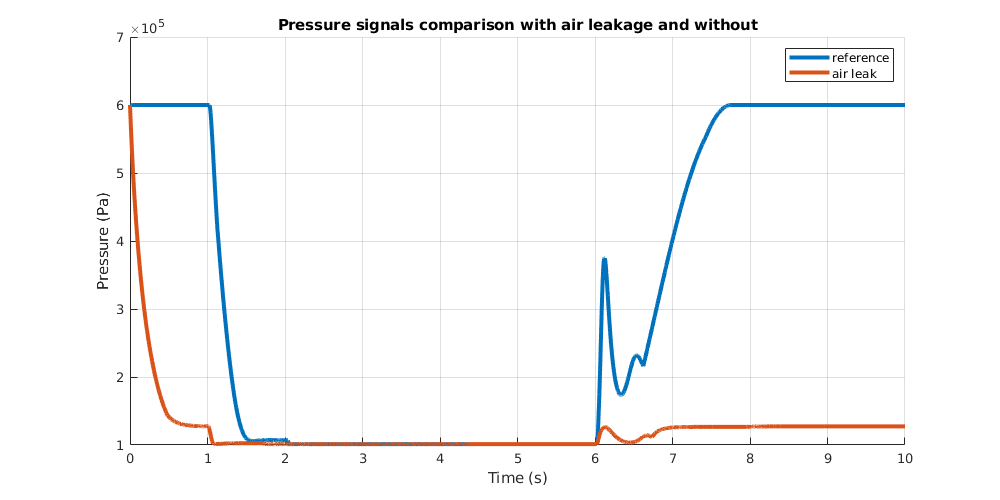
\includegraphics[width=1\textwidth]{pressure_air_leak.png}
    \caption{Development of pressure in the chamber with air leakage}
    \label{fig:pressure_air_leak}
\end{figure}

This fault was modeled on a simulation model with different dynamics of
coefficient C development in the range $C_{al} \in (10^{-10}, 10^{-6})$. The following sections describe how
this data can be used to design RUL estimation.


\subsection{RUL}

The dataset contains 25 simulations, each with a various number of cycles
and different dynamics of air leakage development. After CI extraction in
the form of shape factor figure, \ref{fig:rul_ci} represents the
development of each simulation.

\begin{figure}[h!]
    \centering
    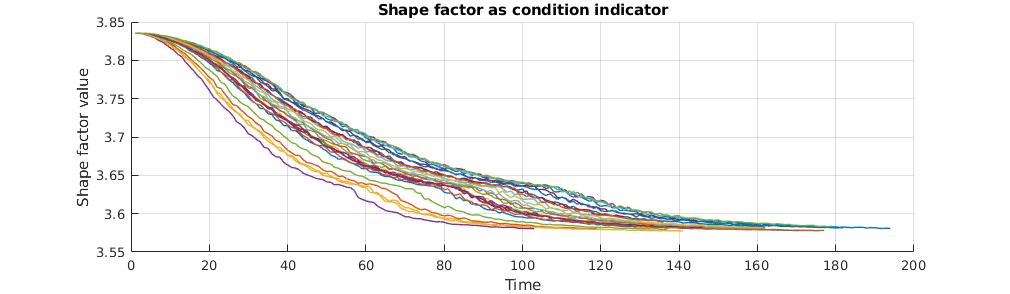
\includegraphics[width=1\textwidth]{rul_ci.png}
    \caption{Development of condition indicator}
    \label{fig:rul_ci}
\end{figure}

\paragraph{Prognostic CI} For RUL algorithm development, prognostic CI is
used. The prognostic CI can be any parameter that represents the
degradation behavior of the system over time. The monotonicity test can be
used for ranking prognostic CI. The shape factor was selected during the
design, but more CIs showed promising results in this particular case.



\paragraph{RUL Models}

Residual similarity, pairwise similarity and linear degradation models were
used for data experiments.


Figure \ref{fig:rul_simil_perfoms} presents results of the residual
similarity model, results of RUL estimation satisfying.  Pairwise
similarity model finding degradation path that is the most correlated to
test data. The residual similarity model fits an ARMA (Autoregressive
Moving Average Model) model on the train data and then computes the
residuals between predicted data from the ARMA model and the test data. The
pairwise similarity model on the generated dataset shows similar results as
the residual similarity model.



\begin{figure}
    \centering
    \begin{subfigure}[b]{0.55\textwidth}
        \centering
        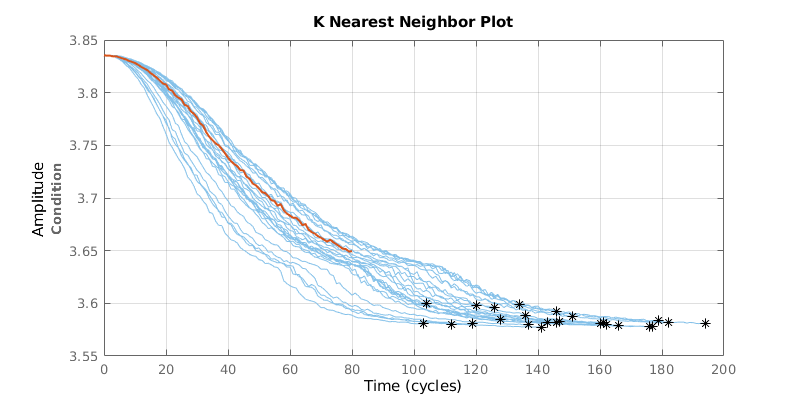
\includegraphics[width=1.2\textwidth]{rul_resid_model_knn.png}
        \caption{Test vs train path development}
        \label{fig:rul_path}
    \end{subfigure}
    \hfill
    \begin{subfigure}[b]{0.4\textwidth}
        \centering
        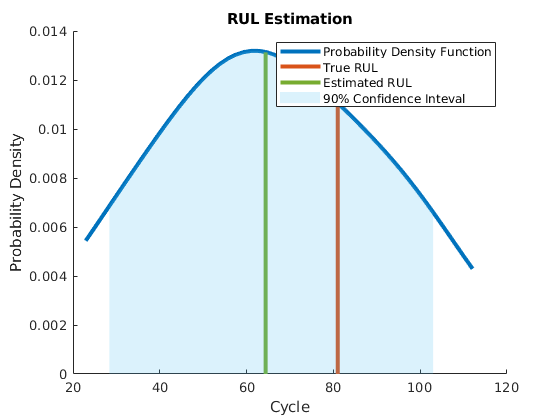
\includegraphics[width=1.1\textwidth]{rul_resid_model_pdf.png}
        \caption{Probability density function estimated RUL}
        \label{fig:rul_pdf}
    \end{subfigure}
    \caption{Residual similarity model performance}
    \label{fig:rul_simil_perfoms}
\end{figure}


Due to figure \ref{fig:rul_ci}, we can determine a safe threshold that we do not want
to exceed and then use the degradation model. In this case, a linear
degradation model was used. This model creates a linear degradation profile
to evaluate the RUL. The results of the linear degradation model are pretty
good \ref{fig:rul_deg_performs}. Predicted RUL shows a deviation from the true RUL of about 10 \%, which
is more than sufficient in this case.

\begin{figure}[h!]
    \centering
    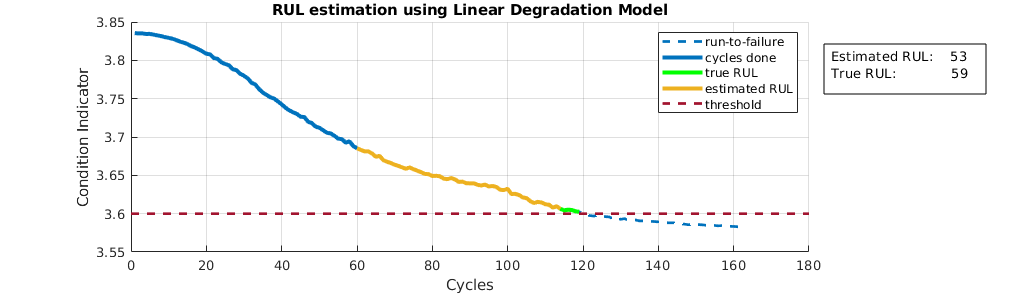
\includegraphics[width=1\textwidth]{rul_final.png}
    \caption{Linear degradation model performance}
    \label{fig:rul_deg_preforms}
\end{figure}


\section{Summary}
A simulation model is a powerful tool for the development of the PdM
algorithm. The possibility of generating unavailable or difficult to
collect data gives an advantage for implementing robust and efficient
algorithms. Since the signal-based method has shown perfect results on the
pneumatic pistol application, using model-based methods such as a residual
estimation seems unnecessary.
